\chapter{\label{chap:chi2}$\rchi^2$ Distribution}
The $\rchi^2_k$ distribution is a non-symmetric distribution with support in the interval $(0,\infty)$, defined for $k=1,2,\ldots$ degrees of freedom as
\begin{equation}
\rchi^2_k(x) = \frac{x^{k/2-1} e^{-\frac{x}{2}}}{2^{k/2} \Gamma(k/2)} \,.
\label{eq:chi2-pdf}
\end{equation}
The cumulative distribution of $\rchi^2$ is surprisingly similar to luck for the $k$ degree-of-freedom normal distribution (\ref{eq:normal-luck-as-integral}),
\begin{equation}
\CDF[\rchi^2_k](x) = \int_0^x \rchi^2_k(y) \, dy = \frac{\gamma(k/2,x/2)}{\Gamma(k/2)} \,.
\label{eq:chi2-cdf}
\end{equation}
For this distribution, the $p$-value is usually the tail integral.  That is,
\begin{equation}
p\text{-value}=1-\CDF[\rchi^2_k](x) \,.
\end{equation}
For $k=1$ and $k=2$ this distribution is monotonically decreasing, and so the luck is just the cumulative distribution function:
\begin{equation}
L[\rchi^2_k](x) = \CDF[\rchi^2_k](x) \text{, when $k=1$ or $k=2$.}
\end{equation}

However, for $k > 2$, the distribution has a single maximum at $x=k-2$ and is otherwise monotonic.  So the luck of an outcome is the integral of the PDF \ref{eq:chi2-pdf} between the observation $x$ and what we call the conjugate point $x^*$ where the distribution values are equal.  This is illustrated in Figure~\ref{fig:chi2-conj} for $k=4$ and $x=5$.
\begin{figure}
\begin{center}
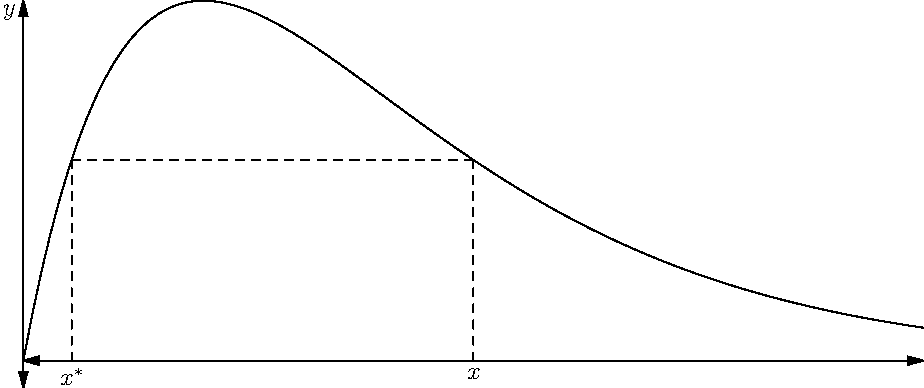
\includegraphics[width=0.75\linewidth]{graphics/chi2-conj.pdf}
\end{center}
\caption{Illustration of the $x^*$ conjugate for the $\rchi^2_4$ distribution at $x=5$.  The conjugate point has the same probability as the original: $\rchi^2_4(x)=\rchi^2_4(x^*)$.  For $x=5$, $x^* \approx 0.5368$.}
\label{fig:chi2-conj}
\end{figure}

There is no algebraic solution for $x^*$, but $\rchi^2_k$ is a smooth curve and so a Newton iteration works well on the logarithmic problem:
\begin{equation}
\log \rchi^2_k(x^*)-\log \rchi^2_k(x) = 0\,.
\end{equation}

A suitable initial guess is to reflect the $x$ around the maximum point, which is asymptotically correct for points near the maximum, but then bound the root from below using the leading order approximation for small $x$,
\begin{align}
x^*_{\text{reflect}} &= \max(0,2\sqrt{k-2}-\sqrt{x})^2 \,. \\
x^*_{\text{lower\_bound}} &= \left[ \rchi^2_k(x) 2^{k/2} \Gamma(k/2) \right]^{\frac{1}{k/2-1}} \\
\intertext{and}
x^*_0 &= \max(x^*_{\text{reflect}},x^*_{\text{lower\_bound}}) \,.
\end{align}

For $x \neq k-2$, the root can quickly be found using the Newton iteration:
\begin{equation}
x^*_{n+1}  = x^*_{n} + \frac{2 x^*_{n}}{x^*_{n}-(k-2)} \left[\log \rchi^2_k(x^*_{n})-\log \rchi^2(x) \right] \,.
\end{equation}

With $x^* = \lim_{n\rightarrow \infty} x_n^*$, luck for $k>2$ can be defined by,
\begin{equation}
L[\rchi^2_k](x)=\left|\CDF[\rchi^2_k](x) - \CDF[\rchi^2_k](x^*)\right| \,.
\end{equation}

A plot of luck $L$ vs $p$-value for $\rchi^2_4$ is given in Figure~\ref{fig:chi2}.
\begin{figure}
\begin{center}
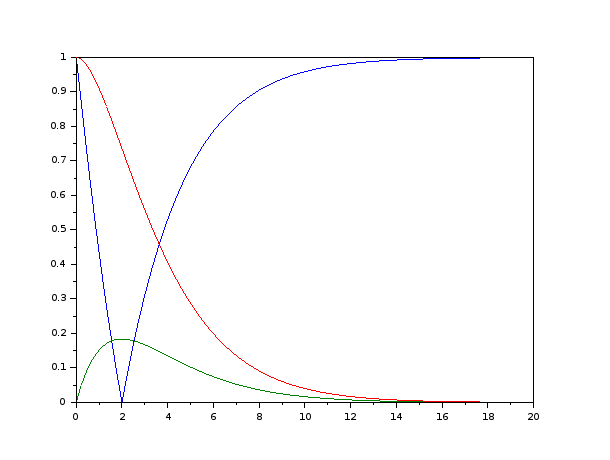
\includegraphics[width=0.75\linewidth]{img/chi2.png}
\end{center}
\caption{$p$-value (red) vs $L$ (blue) for the $\rchi^2$ distribution for $k=4$ (in green).  There is no simple relationship between $L$ and $p$.}
\label{fig:chi2}
\end{figure}

\section{Approximating $L[\rchi^2_k]$.}
A surprisingly good approximation for $L[\rchi^2_k]$ comes from the following observations:
\begin{itemize}
\item Luck is zero at the maximum $x=k-2$.
  \item The tail of the distribution is $O(\erf(\sqrt{x}))$.
\end{itemize}
This suggests
\begin{equation}
  L[\rchi^2_k](x)\approx \erf \left|\sqrt{x}-\sqrt{k-2}\right| \,.
  \label{eq:chi2-luck-est}
\end{equation}
A plot of this estimate vs the numerial solution for large $k$ is given in Figure~\ref{fig:chi2est}.

\begin{figure}
\begin{center}
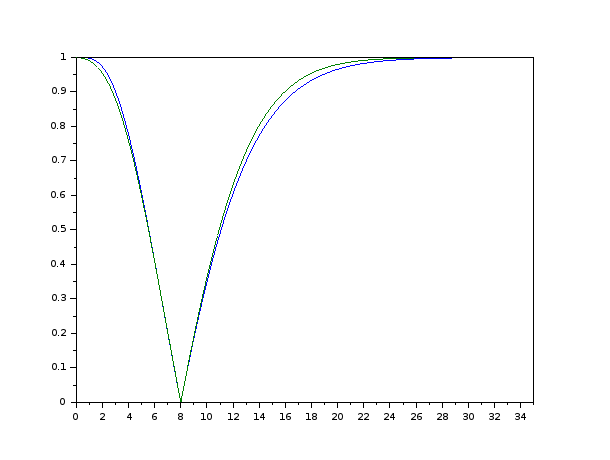
\includegraphics[width=0.75\linewidth]{img/chi2est10.png}
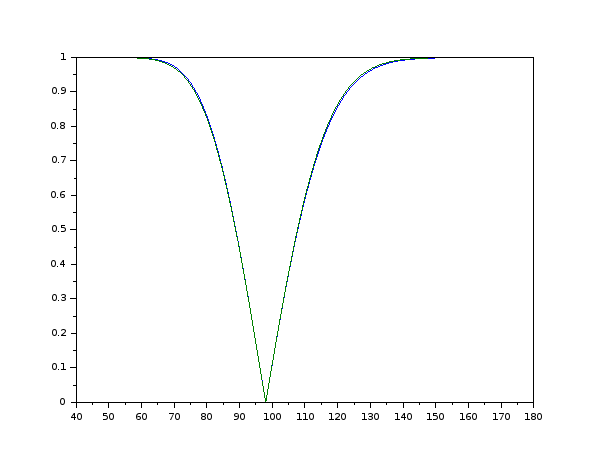
\includegraphics[width=0.75\linewidth]{img/chi2est100.png}
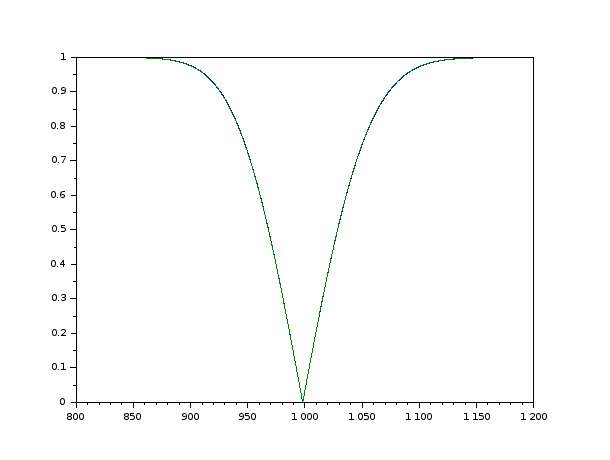
\includegraphics[width=0.75\linewidth]{img/chi2est1000.png}
\end{center}
\caption{$L$ vs $Lestimate$ for $k=10$, $100$, and $1,000$.}
\label{fig:chi2est}
\end{figure}

\section{Scilab reference code}
In order to avoid division by zero, we need a utility function which maps
values away from zero defined by
\begin{equation}
\text{nonzero}_{\varepsilon}(x)=\begin{cases}
x &\text{if }x \notin [-\varepsilon,\varepsilon] \,, \\
-\varepsilon &\text{if }x \in [-\varepsilon,0) \,, \\
\varepsilon &\text{if }x \in [0,\varepsilon] \,. \\
\end{cases}
\end{equation}
Figure~\ref{fig:nonzero} gives a listing in scilab.
\begin{figure}
\caption{\label{fig:nonzero}Scilab utility function to avoid zero}
\lstset{language=Scilab}
\begin{lstlisting}
function y=nonzero(x,eps) 
  y=x .* bool2s((x < -eps) | (eps < x)) + ...
    -eps*bool2s((-eps <= x) & (x < 0))+ ...
     eps*bool2s((0 <= x) & (x <= eps));
endfunction
\end{lstlisting}
\end{figure}

\begin{figure}
\caption{\label{fig:chi2probln}Scilab function to compute $\log \rchi^2_k(x)$}
\lstset{language=Scilab}
\begin{lstlisting}
function lnp=chi2probln(x,k)
  lnx=log(nonzero(x,number_properties('tiny')));
  lnp=lnx.*(k/2-1)-x./2-((k/2)*log(2)+gammaln(k/2));
endfunction
\end{lstlisting}
\end{figure}

\begin{figure}
\caption{\label{fig:chi2cdf}Scilab function to compute $P=\CDF[\rchi^2_k](x)$ and $Q=1-P$}
\lstset{language=Scilab}
\begin{lstlisting}
function [P,Q]=chi2cdf(x,k)
  [dim,nsamps]=size(x);
  one=ones(1,nsamps);
  [P,Q]=cdfgam("PQ",x./2,k/2*one,one);
endfunction
\end{lstlisting}
\end{figure}

\begin{figure}
\caption{\label{fig:chi2conj}Scilab function to compute $x^*$ for the $\rchi^2_k$ distribution.}
\lstset{language=Scilab}
\begin{lstlisting}
function y=chi2conj(x,k)
  [df,nsamps]=size(x);
  lnp=chi2probln(x,k);
  y0=exp((1/(k/2-1))*(lnp+(k/2)*log(2)+gammaln(k/2)));
  y0=max(y0,max(0,2*sqrt(k-2)-sqrt(x)) .^ 2);
  y=y0;
  iterate=%T;
  i=0;
  cutoff=sqrt(%eps);
  while (iterate)
    z=y;
    df=chi2probln(z,k)-lnp;
    dln=2*z ./ nonzero(z-k+2,cutoff);
    y = z +  dln .* df;
    i=i+1;
    iterate = (i<1000) & or(abs(df)>cutoff);
  end
endfunction
\end{lstlisting}
\end{figure}

\begin{figure}
\caption{\label{fig:chi2luck}Scilab function to compute $L=L[\rchi^2_k](x)$ and $U=1-L$.}
\lstset{language=Scilab}
\begin{lstlisting}
function [L,U]=chi2luck(x,k)
  y=chi2conj(x,k);
  [a,b]=chi2cdf(x,k);
  [A,B]=chi2cdf(y,k);
  L=abs(B-b);
  U=(A+b).*bool2s(x>=y)+(a+B).*bool2s(x<y);
endfunction
\end{lstlisting}
\end{figure}

\section{Summary}
\begin{itemize}
\item $\rchi^2_k$ is a common non-symmetric distribution (\ref{eq:chi2-pdf}):
  \begin{equation*}
\rchi^2_k(x) = \frac{x^{k/2-1} e^{-\frac{x}{2}}}{2^{k/2} \Gamma(k/2)} \,.    
  \end{equation*}
\item For $k=1$ or $k=2$ degrees of freedom it is monotonic.  But for $k>2$ it has a single maximum at $x=k-2$.
\item We define $x^*$ as the conjugate point to $x$:
  \begin{equation*}
    x^* = \begin{cases}
      \text{Solution $x^* \neq x$ to $\rchi^2_k(x^*)=\rchi^2_k(x)$}
      & \text{if $k>2$ and $x \neq k-2$.} \\
      k-2 & \text{if $k>2$ and $x = k-2$.} \\
      0 & \text{if $k \in \{1,2\}$ and $x > 0$.} \\
      +\infty & \text{if $k \in \{1,2\}$ and $x = 0$.}
    \end{cases}
  \end{equation*}
  This can be found using standard numerical techniques.
\item With the conjugate point,
  \begin{equation*}
    L[\rchi^2_k](x)=\left| CDF[\rchi^2_k](x^*) -CDF[\rchi^2_k](x) \right|
  \end{equation*}
\item For large $k$ (\ref{eq:chi2-luck-est}),
  \begin{equation*}
  L[\rchi^2_k](x)\approx \erf \left|\sqrt{x}-\sqrt{k-2}\right| \,.    
  \end{equation*}
\end{itemize}

